\chapter{Algebraic complexity classes} \label{chap-vpvnp}

Valiant \cite{v79} defined two algebraic complexity classes that can be thought of as analogues of the boolean classes $\P$ and $\NP$. 
This chapter focuses on their definitions, and some important properties related to the polynomial families $\Det_n$ and $\Perm_n$. 

\section{Definition of classes}

Recall that $\P$ is\footnote{if one is to be more precise, this is $\P/\poly$ or non-uniform $\P$. 
But in this article, we shall be interested only in the non-uniform versions since we mainly deal with circuit sizes.} the class of boolean functions that can be computed by circuits of polynomial size. 
As any boolean function can be expressed as a multilinear\footnote{a polynomial where the degree in any variable is bounded by $1$} polynomial, an analogue of this in the arithmetic world could be multilinear polynomials $f(x_1,\dots, x_n)$ that can be computed by arithmetic circuits of size $\poly(n)$. 
However, unlike in the boolean world, the polynomial $x^2$ is not equal to the polynomial $x$ as we are dealing with formal polynomials. 
Valiant's definition of $\VP$ was the class of the class of ``low degree'' polynomials that can be computed by circuits of small size. 

\begin{definition}[Valiant's $\P$]\label{defn:vp}
The class $\VP$ refers to the set of polynomials $f(x_1,\dots, x_n)$ of \emph{degree $\poly(n)$} that can be computed by arithmetic circuits of size $\poly(n)$. 
\end{definition}

In the literature, one also encounters classes such as $\mathsf{VBP}$ and $\mathsf{VF}$ that correspond to polynomials computed by polynomial-sized ABP and formulas respectively. 
These are subclasses of $\VP$ by definition. 


\subsection*{More on the low-degree restriction}

But should the analogue of $\VP$ not be the class of polynomials that are computable by $\poly(n)$-sized arithmetic circuits, that include such polynomials of very large degree? 
We can indeed compute polynomials of very large degree, such as a circuit that is a chain of $s$ multiplication gates thus computing a polynomial of degree $\mathrm{exp}(s)$ (by repeated squaring). 
Let us first take a moment to understand why the additional restriction of ``low-degree'' in the above definition of $\VP$ was imposed. 
There are several intuitive reasons for this, and this ``restricted'' definition also yields beautiful structural results. 
This discussion is from an answer by Joshua Grochow on \texttt{cstheory.SE} \cite{gro:SE} to shed more light on the above definition. 

\begin{enumerate}

\item Every boolean function can be expressed as a multilinear polynomial. 
Multilinear polynomials are of course polynomials of ``low degree''. 

\item Much of the earlier work were based on understanding formula size. 
In the case of arithmetic formulas, the degree cannot be more than the size of the formula. 
If a polynomial is computed by a $\poly(n)$ sized formula, then its degree must be bounded by $\poly(n)$ too. 

\item Most interesting polynomials, such as $\Det_n$ or $\Perm_n$, are in fact of low degree. 
Once we choose to deal with only polynomials of low degree, the above definition does not have any restriction on the circuit used to compute it (besides its size). 
It is certainly possible that intermediate computations of the circuit could involve very large degree polynomials. 

However, as we shall soon see, Strassen's result shows that such high degree computations may be eliminated with just an $O(\deg^2)$ increase in size. 
Dealing with low-degree circuits also makes the class robust under this transformation. 
Eliminating division gates also only incurs an $O(\deg^2)$ increase in size. 

\item Without this restriction, cannot hope to show that $\Det_n$ or $\Perm_n$ is ``complete'' for such classes, or the numerous structural results such as depth reduction that we have. 

\end{enumerate}

Having said that, there is also a notion of ``degree'' in a boolean circuit that is defined syntactically as follows:
 \begin{quote}
   Degree of all leaves is $1$. 

   For any OR gate, the degree is the maximum of the degree of its children. 

   For any AND gate, the degree is the sum of the degrees of its children. 
 \end{quote}
The class boolean functions that can be computed by poly-sized poly-degree circuits coincide with a class called $\mathsf{LOGCFL}$ or $\mathsf{SAC}^1$. 
With this notion, one might say that $\VP$ is really an analogue of $\mathsf{SAC}^1$.\\


We now move on to the arithmetic analogue of the class $\NP$. 
Recall that the class $\NP$ may be defined as the set of all boolean functions $f(x_1,\dots, x_n)$ such that there is some $g(x_1,\dots, x_n, y_1,\dots, y_m)$ with $m = \poly(n)$ such that 
\[
f(x_1,\dots, x_n)\spaced{=} \bigvee_{\veca \in \inbrace{0,1}^m}  g(x_1,\dots, x_n, a_1,\dots, a_m)
\]
Valiant's $\NP$ is defined analogously by replacing the OR by a sum. 

\begin{definition}[Valiant's $\NP$]\label{defn:vnp}
The class $\VNP$ is defined to be the set of polynomials $f(x_1,\dots, x_n)$ such that there is some $g(x_1,\dots, g_n, y_1,\dots, y_m) \in \VP$ with $m = \poly(n)$ such that 
\[
f(x_1,\dots, x_n)\spaced{=} \sum_{\veca \in \inbrace{0,1}^m}  g(x_1,\dots, x_n, a_1,\dots, a_m)
\]
\end{definition}

It follows from definitions that $\mathsf{VF} \subseteq \mathsf{VBP} \subseteq \VP \subseteq \VNP$. 
We do not know if any of the containments is strict (although it is widely believed that all of them are). 

\section{Some properties of these classes}

We shall state a few properties of these classes here. 
For a more extensive treatment, B\"{u}rgisser's book \cite{bur00} has a comprehensive study of these classes and a lot of the proofs presented in this chapter are based on the description in his book. \\

Valiant~\cite{v79} presented a very useful sufficient condition to show that a given polynomial is in $\VNP$. 

\begin{theorem}[Valiant's Criterion] \label{thm:val-criterion}
Let $f = \sum_\vece c(\vece) \cdot x_1^{e_1}\dots x_n^{e_n}$. 
Suppose the function $\varphi$ that takes as input the exponent vector $\vece = (e_1,\dots, e_n)$ and outputs the coefficient $c(\vece)$ is in the class $\#\P/\poly$, then $f \in \VNP$. 
\end{theorem}

Thus in particular, if we compute the coefficient for a given monomial in polynomial time, then the polynomial is in $\VNP$. 

\begin{corollary}
The polynomials $\Perm_n$ and $\NW_{n,m,d}$ are in $\VNP$. 
\end{corollary}

As stated in \autoref{defn:vnp}, the polynomial $g(x_1,\dots, x_n, y_1,\dots, y_m) \in \VP$. 
However, a subsequent paper of Valiant~\cite{v82} showed that we may assume with loss of generality that $g \in \mathsf{VF}$, that is $g$ is computable by a small formula. 
This is similar to the fact that counting solutions of 3-\textsf{CNF} instance, which is a formula, is as hard as counting solutions of any polynomial sized boolean circuit. 
We state this result here, and a proof may be found in B\"urgisser's book \cite{bur00}. 

\begin{theorem}\label{thm:vnp-formula}
For any $f(x_1,\dots, x_n)\in \VNP$, there is a $g(x_1,\dots, x_n, y_1,\dots, y_m)$ that can be computed by a $\poly(n)$ sized \emph{formula} such that 
\[
f(x_1,\dots, x_n)\spaced{=} \sum_{\veca \in \inbrace{0,1}^m} g(x_1,\dots, x_n, a_1,\dots, a_m)
\]
\end{theorem}

\section{Reductions and completeness}

For polynomials, the most natural form of reductions are via \emph{projections}. 
We shall say that a polynomial $f$ \emph{reduces} to $g$ via projections if $g$ may be obtained by setting substituting variables of $f$ to other variables or field constants. 
Under such reductions, do we have natural complete polynomials for the classes $\VP$ and $\VNP$? 
Valiant \cite{v79} showed that the $\Det_n$ and $\Perm_n$ are (almost) complete for the classes $\VP$ and $\VNP$ respectively. 
We shall see the proof of this in this section. 

\begin{theorem}[\cite{v79}]\label{thm:vp}
If $f$ is a polynomial computed by an ABP of size $s$, then $f$ reduces to $\Det_n$ via projections for $n = \poly(s)$. 
\end{theorem}
\begin{theorem}[\cite{v79}]\label{thm:vnp}
Over any field $\F$ of characteristic not equal to $2$, the polynomial $\Perm_n$ is \emph{complete} for the class $\mathsf{VNP}$ under projections.
\end{theorem}

\subsection{Formulas to determinants}\label{sec:formula-to-dets}

Let us first show that any polynomial sized arithmetic formula can be expressed as determinant of a small matrix.
In fact, all matrices that we shall be building this way will have the following structure, and this would be important.\\

\begin{center}
\begin{tikzpicture}
\node at  (-1.5,1.5) {$f \quad = \quad \Det$};
\draw (0,0) rectangle (3,3);
\node at (0.25,0.25) {1};
\node at (2.75,0.25) {0};
\node at (0.25,2.75) {0};
\node[text=red] at (0.75,2.25) {$\ast$};
\node[text=red] at (2.25,0.75) {$\ast$};
\draw[dotted] (2,1) -- (1,2);
\draw (0.75,2.75) -- (2.75,2.75) -- (2.75,0.75) -- cycle;
\node[text=red] at (2.1,2.1) {$\ast$};
\begin{scope}[shift={(8,0)}]
\node at  (-1.5,1.5) {$g \quad = \quad \Det$};
\draw (0,0) rectangle (3,3);
\node at (0.25,0.25) {1};
\node at (2.75,0.25) {0};
\node at (0.25,2.75) {0};
\node[text=blue] at (0.75,2.25) {$\ast$};
\node[text=blue] at (2.25,0.75) {$\ast$};
\draw[dotted] (2,1) -- (1,2);
\draw (0.75,2.75) -- (2.75,2.75) -- (2.75,0.75) -- cycle;
\node[text=blue] at (2.1,2.1) {$\ast$};
\end{scope}
\end{tikzpicture}
\end{center}
We shall assume that the matrices for $f$ and $g$ have the same size (it is easy to pad the matrices while preserving the structure). 

\subsection*{Multiplication}

\begin{center}
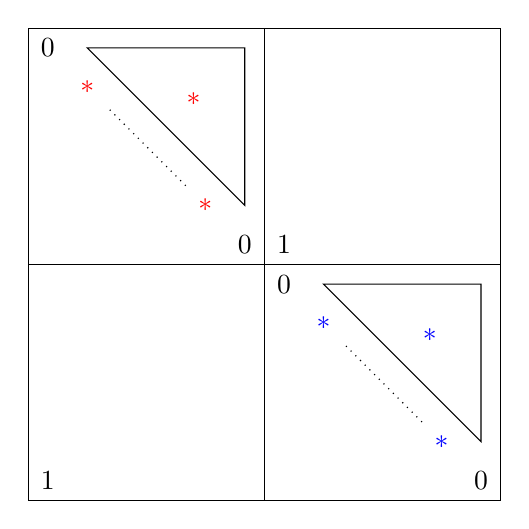
\begin{tikzpicture}
\draw (0,-3) rectangle (6,3);
\draw (0,0) rectangle (3,3);
\node at (2.75,0.25) {0};
\node at (0.25,2.75) {0};
\node[text=red] at (0.75,2.25) {$\ast$};
\node[text=red] at (2.25,0.75) {$\ast$};
\draw[dotted] (2,1) -- (1,2);
\draw (0.75,2.75) -- (2.75,2.75) -- (2.75,0.75) -- cycle;
\node[text=red] at (2.1,2.1) {$\ast$};
\begin{scope}[shift={(3,-3)}]
\draw (0,0) rectangle (3,3);
\node at (2.75,0.25) {0};
\node at (0.25,2.75) {0};
\node[text=blue] at (0.75,2.25) {$\ast$};
\node[text=blue] at (2.25,0.75) {$\ast$};
\draw[dotted] (2,1) -- (1,2);
\draw (0.75,2.75) -- (2.75,2.75) -- (2.75,0.75) -- cycle;
\node[text=blue] at (2.1,2.1) {$\ast$};
\end{scope}
\node at (0.25,-2.75) {1};
\node at (3.25,0.25) {1};
\end{tikzpicture}
\end{center}

\subsection*{Addition}

\begin{center}
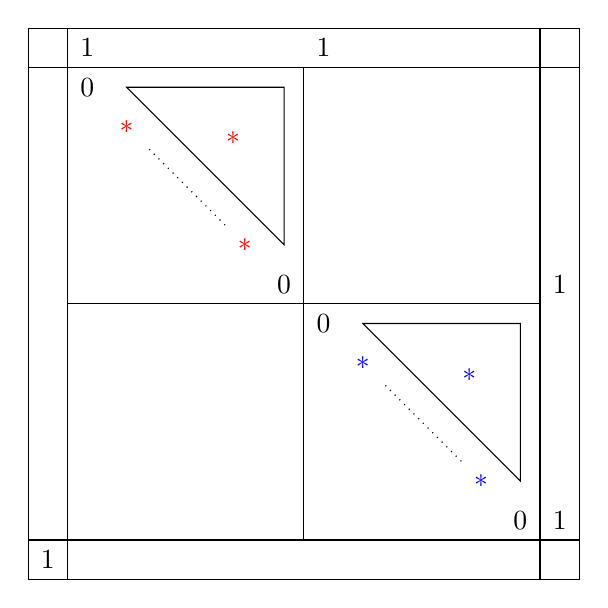
\begin{tikzpicture}

\draw (-0.5,-3.5) rectangle (0,3.5);
\draw (6,-3.5) rectangle (6.5,3.5);
\draw (6,3) rectangle (0,3.5);
\draw (0,-3.5) rectangle (6,3);

\draw (-0.5,-3) rectangle (6.5,3);
\draw (0,0) rectangle (3,3);
\node at (2.75,0.25) {0};
\node at (0.25,2.75) {0};
\node[text=red] at (0.75,2.25) {$\ast$};
\node[text=red] at (2.25,0.75) {$\ast$};
\draw[dotted] (2,1) -- (1,2);
\draw (0.75,2.75) -- (2.75,2.75) -- (2.75,0.75) -- cycle;
\node[text=red] at (2.1,2.1) {$\ast$};
\begin{scope}[shift={(3,-3)}]
\draw (0,0) rectangle (3,3);
\node at (2.75,0.25) {0};
\node at (0.25,2.75) {0};
\node[text=blue] at (0.75,2.25) {$\ast$};
\node[text=blue] at (2.25,0.75) {$\ast$};
\draw[dotted] (2,1) -- (1,2);
\draw (0.75,2.75) -- (2.75,2.75) -- (2.75,0.75) -- cycle;
\node[text=blue] at (2.1,2.1) {$\ast$};
\end{scope}
\node at (-0.25,-3.25) {1};
\node at (0.25,3.25) {1};
\node at (3.25,3.25) {1};
\node at (6.25,0.25) {1};
\node at (6.25,-2.75) {1};
\end{tikzpicture}
\end{center}

We leave it to as an exercise to check that this indeed works. This may seem bizarre at first but there is indeed a method to this. To understand that, we must realise that there is a graph theoretic way to understand $\Det_n$ and $\Perm_n$. 

\subsubsection*{Graph theoretic representation of $\Det_n$ and $\Perm_n$}

Let us think of an $n\times n$ symbolic matrix as an adjacency matrix of a directed graph $G$ with the edge from $i$ to $j$ having weight $x_{ij}$. 
Then every monomial of $\Det_n$ or $\Perm_n$ corresponds to a permutation $\sigma$, and the corresponding edges in the graph $G$ form a \emph{cycle cover} i.e. a partition of the vertices of $G$ into disjoint cycles. 
The weight of a cycle-cover shall be defined as the product of weights of the edges constituting the cycles, and the sign of the cycle cover shall be the sign of the permutation $\sigma$. 
This allows us to write $\Det_n$ and $\Perm_n$ as
\begin{eqnarray*}
\det(G) & = & \sum_{C\in \mathrm{CycleCovers}(G)} wt(C) \cdot \mathrm{sign}(C)\\
\mathrm{perm}(G) & = & \sum_{C\in \mathrm{CycleCovers}(G)} wt(C) \\
\end{eqnarray*}

\subsection{ABPs reduce to $\Det_n$}

We shall now show that for any $f$ computable by an ABP, there is a matrix  $A$ each of whose entries are either variables of constants such that $\det(A) = f$. 
Since any ABP is a projection of the polynomial $\IMM_{n,d}$, we shall show that we can construct a matrix  $A$  such that $\det(A) = \IMM_{n,d}$. \\

Consider the graph $G$ underlying the ABP that corresponds to the polynomial $\IMM_{n,d}$. 
Let $s$ and $t$ be the unique source and sink vertices respectively. 
Every path from $s\leadsto t$ corresponds to a single monomial of $\IMM_{n,d}$ of degree $d$. 
We shall now modify the graph slightly such that each such $s\leadsto t$ path would map to a unique cycle cover:

\begin{quote}
  To the graph $G$, add an edge with weight $1$ from $t$ to $s$. 

  Further, for all nodes except $s$ and $t$, add a self-loop of weight $1$. 
\end{quote}

Let $A$ be the adjacency matrix of this new graph $G'$. 
The claim is that $\det(A)$ is either $\IMM_{n,d}$ or $\IMM_{n,d}$. 
To see this observe that all cycle covers of $G'$ must consist of a single $s\leadsto t$ path that loops back to $s$ via the edge $t\rightarrow s$ that we added, and self-loops on all excluded vertices. 
Further, since all $s\leadsto t$ paths in $G$ were of the same length, it is easy to check that all the cycle covers have the same sign. 
Thus $\IMM_{n,d}$ does indeed reduce to $\Det_m$ for $m = \poly(n)$. \qed {\footnotesize (\autoref{thm:vp})}\\

\begin{exercise}
Look back at the construction in \autoref{sec:formula-to-dets} to convince yourself that the determinants are indeed $f \cdot g$ and $f + g$. 
\end{exercise}


\subsection{$\Det_n$ can be computed by ABPs}

A result that is often stated but not proved explicitly is a polynomial sized circuit for $\Det_n$. 
This is often attributed by Berkowitz \cite{Berk84}. 
In fact, $\Det_n$ has a polynomial sized ABP and this construction is due to Mahajan and Vinay~\cite{mv97} based on \emph{clow sequences}. 
The construction is really neat and we shall describe the ABP explicitly here. 

\[
\Det_n \spaced{=} \abs{\begin{array}{ccc}
x_{11} & \dots & x_{1n}\\
\vdots & \ddots & \vdots \\
x_{n1} & \dots & x_{nn}
\end{array}
}\]

If the symbolic matrix on the RHS is the adjacency matrix of an $n$-vertex graph, then the determinant is just the sum of weighted signed cycle-covers of the graph. 
A natural approach compute this via an ABP is to somehow compute each cycle cover on one path of the ABP. 
Unfortunately, if one were to try the \naive approach of building a cycle cover over many layers, to decide what our next vertex should be we are forced to remember the entire partial construction thus far. 
This ends up yielding an ABP with super-polynomial width (the width intuitively corresponds to the memory required). 

The key insight of Mahajan and Vinay was to relax the notion of cycle covers to something weaker that can be built with less memory, to what they called \emph{clow sequences}. 

\begin{definition}[Clow Sequences]
Label the vertices of the graph as $1,\dots, n$. 
A clow  of length $\ell$ is a closed walk on the graph $G$ of length $\ell$ such as $v_1,\dots, v_\ell,v_1$ such that $v_1 < v_i$ for all $i=2,\dots, \ell$. 
We shall also refer to $v_1$ as the \emph{head of the clow}. 

In other words, the head of a clow is the smallest vertex of the walk, and the head does not repeat in a clow (although other vertices can). 

A clow sequence is a sequence of clows $(C_1,\dots, C_r)$ that additionally satisfy $\mathrm{head}(C_1) < \dots < \mathrm{head}(C_r)$. 

The length of a clow sequence is the sum of the lengths of the clows that it comprises of. 
The weight of a clow sequence is just the product of weights of the edges it comprises of. 
Also, the sign of a clow sequence of length $\ell$ that comprises of $r$ clows is $(-1)^{\ell + r}$. 
\end{definition}

Any cycle cover is of course a clow sequence. 
Further, the sign of the cycle cover matches the above definition of the sign of a clow sequence. 
But there are many clow sequences that visit some vertices multiple times, and hence not cycle covers. 
However, Mahajan and Vinay show that the sum of signed-weights of all clow sequences also yields the determinant. 

\begin{lemma}[\cite{mv97}]\label{lem:mv-clowseq} If $A_G$ is the adjacency matrix of a graph $G$, then
\begin{eqnarray*}
\det(A_G) & = &  \sum_{C \in \mathrm{CycleCover(G)}} wt(C) \cdot \mathrm{sign}(C) \spaced{=} \det(A_G)\\
& = & \sum_{C \in \mathrm{ClowSequence(G)}} wt(C) \cdot \mathrm{sign}(C)
\end{eqnarray*}
\end{lemma}

They prove this by showing that the set of clow sequences that are not cycle covers can partitioned into pairs $(C_1,C_2)$ such that $wt(C_1) = wt(C_2)$ and $\mathrm{sign}(C_1) = - \mathrm{sign}(C_2)$. 
We shall see an explicit proof of this shortly, but first let us see why this yields an ABP. \\

The ABP consists of $n+1$ layers labelled as layer $1,\dots, n+1$. 
Besides layer $1$ and $n+1$, every other layer $\ell$ consists of $\Theta(n^2)$ nodes that we shall label as $v_{i,j}^{(\ell)}$ for $1\leq i\leq j\leq n$. 
It is best to think of $i$ as representing the \emph{head of the current clow}, and $j$ as the \emph{current vertex in the clow}. 
The length of the partial clow sequence constructed so far is captured by the layer index $\ell$. 

The first layer consists of a single vertex that we shall call $s = v_{1,1}^{(1)}$ (to maintain the same notation)  and the last layer consists of a single vertex that we shall call $t$. 
The edges between layers, and the weights are defined as follows:

\begin{enumerate}
\item For each node $v_{i,j}^{(\ell)}$ in layer $\ell \in [n]$, there is an edge to vertex $v_{i,k}^{(\ell+1)}$ for every $k > i$. 
The weight of this edge is $x_{jk}$. 

(This is like adding vertex $k > i$ to our current clow by taking edge $x_{jk}$. 
The head continues to be $i$, and the current vertex is now $k$. )
\item For each node $v_{i,j}^{(\ell)}$ in layer $\ell \in [n]$, there is an edge to vertex $v_{k,k}^{(\ell+1)}$ for every $k > i$. 
The weight of this edge is $(-x_{ji})$. 

(This is like ending the current clow by taking edge $x_{ji}$ back to the head, and starting a new clow with head as $k$. 
Thus, the head of the current clow is $k$, and the current vertex is also $k$. 
In this process, we increased the number of clows in the sequence by 1 and hence the weight being $(-x_{ji})$ accounts for the sign change as well.)

\item For the last layer, each node $v_{i,j}^{(n)}$ has an edge to $t$ with weight $(-x_{ji})$. 

(This just corresponds to ending the last clow in our sequence.)
\end{enumerate}


\noindent
Summarizing this as a theorem, we have:

\begin{theorem}[\cite{mv97}]\label{thm:det-abp}
The polynomial $\Det_n$ can be computed by an ABP of size $O(n^3)$ over any field $\F$. 
Thus, in particular, $\Det_n$ can be computed by a arithmetic circuit of size $\poly(n)$. 
\end{theorem}


\begin{proofof}{\autoref{lem:mv-clowseq}}
Consider a clow sequence $C = (C_1,\dots, C_r)$ of length $n$, ordered so that $\mathrm{head}(C_1) < \dots < \mathrm{head}(C_r)$. 
If $C$ is \emph{not} a cycle-cover, then some vertex must be repeated in $C$. 
Starting from the last clow and proceeding backwards, let $i$ be an index such that $(C_{i+1},\dots, C_{r})$ is a union of disjoint cycles but $(C_{i},\dots, C_r)$ is not, and let $C_i = (v_1,\dots, v_k)$. 
Let $j$ be the first index that makes the vertex $v_{j}$ show that $(C_i,\dots, C_r)$ not be a union of disjoint cycles. 
Then, exactly one of the two situations must occur:
\begin{description}
 \item[Case 1:] $v_{j} = v_{j'}$ for some $j' < j$,

 \item[Case 2:] $v_{j}$ occurs in one of the cycles $C_{i+1},\dots, C_r$. 
\end{description}

In the first case, the vertices $v_{j'+1},\dots, v_{j}$ are all distinct since $v_j$ was the first occurrence of a repeated node. 
Define a new clow sequence  $\tilde{C}$ obtained by decomposing the clow $C_i$ with two clows $\inparen{(v_1,\dots, v_{j'},v_{j+1},\dots, v_k), (v_{j'},v_{j'+1},\dots,v_{j})}$. 
Note that the second clow $(v_{j'},\dots, v_j)$ is an honest-to-god cycle that does not intersect with any of the cycles $C_{i+1},\dots, C_r$. 
This transformation converts the clow sequence $C$ with $r$ clows to a clow sequence $C'$ of $r+1$ clows and hence $\mathrm{sign}(C) = - \mathrm{sign}(C')$. 

In the second case, we have $v_j \in C_i$ present also in $C_{i'}$ for some $i' > i$. 
Here we shall apply the inverse operation of combining the clows $C_i$ and $C_i'$ at the vertex $j$. 
Formally, let us rotate $C_{i'}$ cyclically so that $C_{i'} = (v_1',\dots, v_k')$ with $v_1' = v_j$. 
The new clow sequence $C'$ shall be constructed by replacing the clows $C_i$ and $C_{i'}$ by a new clow $(v_1,\dots, v_j, v_2',\dots, v_k', v_{j+1},\dots)$. 
Since every vertex in $C_{i'}$ is greater than $\mathrm{head}(C_{i'})$ which is greater than $\mathrm{head}(C_i)$, this process does indeed result in a valid clow. 
Once again, $\mathrm{sign}(C) = - \mathrm{sign}(C')$ as the number of clows in the sequence has reduced by exactly one.\\

\begin{tikzpicture}[->,>=stealth',shorten >=1pt,auto,thick,main node/.style={circle,fill=blue!20,draw,font=\tiny}]
\node at (0,0.5) {\tiny head};
\node[main node] (v1) at (0,0) {1};
\node[main node] (v2) at (-1,-0.7) {2};
\node[main node] (v3) at (-1,-2.3) {7};
\node[main node] (v4) at (0.5,-2.8) {5};
\node[main node] (v5) at (1.5,-2) {4};
\node[main node] (v6) at (1.2,-0.5) {8};


\path[bend right] (v1) edge (v2)
(v2) edge (v3)
(v3) edge (v4)
(v4) edge (v5)
(v5) edge (v6)
(v6) edge (v1);


\node[main node] (v61) at (2.5,-1.5) {3};
\node[main node] (v62) at (3,-2.5) {9};
\node[main node] (v63) at (2,-2.8) {6};

\path[bend left] (v5) edge (v61)
(v61) edge (v62)
(v62) edge (v63)
(v63) edge (v5);
\node at (1,-4) {$(1,2,7,5,4,3,9,6,4,8,1)$};

\node at (8,0.5) {\tiny head};
\node[main node] (u1) at (8,0) {1};
\node[main node] (u2) at (7,-0.7) {2};
\node[main node] (u3) at (7,-2.3) {7};
\node[main node] (u4) at (8.5,-2.8) {5};
\node[main node,draw=red] (u5) at (9.5,-2) {4};
\node[main node] (u6) at (9.2,-0.5) {8};
\path[bend right] (u1) edge (u2)
(u2) edge (u3)
(u3) edge (u4)
(u4) edge (u5)
(u5) edge (u6)
(u6) edge (u1);


\node[main node,draw=red] (u50) at (11.5,-1.5) {4};
\node at (12.5,-0.5) {\tiny head};
\node[main node] (u51) at (12.5,-1) {3};
\node[main node] (u52) at (13,-2) {9};
\node[main node] (u53) at (12,-2.3) {6};
\path[bend left] (u50) edge (u51)
(u51) edge (u52)
(u52) edge (u53)
(u53) edge (u50);
\node at (10,-4) {$(1,2,7,5,4,8,1),(3,9,6,4,3)$};

\node at (5,-2) {\Huge $\Longleftrightarrow$};
\end{tikzpicture}

It is not hard to see that the two operations in the two different cases are exact inverses of each other. 
Thus, this establishes a matching among all clow sequences that are not cycle covers, with every matched pair having opposing signs. 
Thus, the overall contribution of clow sequences that are not cycle covers is zero. 
\end{proofof}


\subsection{Completeness of the permanent}

The $\VNP$ completeness for the permanent is trickier, and uses a very clever gadget. 
The proof described here is a modification of the proof in B\"urgisser's book \cite{bur00}. 
This is the simplest proof that I am aware of currently. \\

Let $f(x_1,\dots, x_n) = \sum_\veca g(x_1,\dots, x_n, a_1,\dots, a_m)$ be in $\VNP$ with $g(\vecx, \vecy)$ computable by a formula of size $s$ (\autoref{thm:vnp-formula}). 
Like in the previous section, we can construct a graph $G$ (with weights being either scalars or variables in $\vecx$ or $\vecy$) such that the sum of weighted cycle covers is equal to $g(\vecx, \vecy)$. 
The goal is to now compute $\sum_\veca g(\vecx, \veca)$. \\

Let us consider a simpler case, where there is a variable $y \in \vecy$ such that there is just one edge in $e_y \in G$ with weight $y$. 
Can we transform the graph $G$ locally to compute $g' = g_{(y=0)} + g_{(y=1)}$? 
Note that since $y$ occurs only once in $G$, we have that $g = y \cdot g_1 + g_0$ where $g_1$ and $g_0$ are independent of $y$. 
Thus, the polynomial $g'$ can be written as $g_1 + 2 g_0$. 
One way to compute this is to transform the graph $G$ so that any cycle-cover of $G$ that includes the edge $e_y$ has the same weight as before, but every cycle-cover that does not include the edge $e_y$ has its weight multiplied by $2$. 
This can be achieved by splitting the edge $e_y$ in the middle with a new vertex $v$ with a self-loop of weight $2$:

\begin{tikzpicture}[->,>=stealth',shorten >=1pt,auto,thick,main node/.style={circle,fill=blue!20,draw}]
\node[main node] (u) at (0,0) {};
\node[main node] (v) at (2,0) {}
edge[<-] node[above] {$y$} (u);
\node (arrow) at (4,0) {\Large $\leadsto$};
\node[main node] (u1) at (6,0) {};
\node[main node] (u2) at (7,0) {}
edge[<-] (u1);
\node[main node] (v1) at (8,0) {}
edge[<-] (u2);
\path[every node/.style={font=\tiny}] (u2) edge [loop above] node {2} (u2);
\end{tikzpicture}

Clearly, any cycle-cover that uses the edge $e_y$ has the same weight, and all other cycle-covers are forced to take the self-loop around the added vertex of weight $2$. 
This allows us to handle graphs $G$ where every variable $y \in \vecy$ occurs only once in $G$. 
The complication arises because there could be multiple edges that has the label $y$. 
We want a way by which we can say that all cycle covers that choose \emph{any} of the $y$-edges have the same weight, but cycle-covers that do not pick any $y$-edge have weight multiplied by $2$. 
The following is a gadget that has similar properties, called \emph{rosette}. 
The diagram below represents the $4$-rosette. 
\begin{center}
\begin{tikzpicture}[->,>=stealth',shorten >=1pt,auto,thick,main node/.style={circle,fill=blue!20,draw}]
\node[main node] (v1) at (0,0) {};
\node[main node] (v2) at (2,0) {};
\node[main node] (v3) at (2,2) {};
\node[main node] (v4) at (0,2) {};

\path[every node/.style={font=\tiny},ultra thick] (v1) edge (v2)
(v2) edge (v3)
(v3) edge (v4)
(v4) edge (v1);

\node[main node] (l1) at (1,-1) {};
\node[main node] (l2) at (3,1) {};
\node[main node] (l3) at (1,3) {};
\node[main node] (l4) at (-1,1) {};

\path[every node/.style={font=\tiny},thick] (l1) edge (v2)
edge [loop below] (l1)
(v2) edge (l2)
(l2) edge[loop right] (l2)
(l2) edge (v3)
(v3) edge (l3)
(l3) edge [loop above] (l3)
(l3) edge (v4)
(v4) edge (l4)
(l4) edge [loop left] (l4)
(l4) edge (v1) 
(v1) edge (l1);
\end{tikzpicture}
\end{center}
The thick edges in the above picture shall be called \emph{connector edges} (these shall play the role of the $y$-edges). 
Note that the rosette has the following two properties:
\begin{enumerate}
\item For any non-empty subset $S$ of the connector edges, there is exactly one cycle-cover of the rosette that includes exactly the set $S$ of the connector-edges. 
\item There are exactly two cycle-covers of the rosette that do not include any connector edge. 
\end{enumerate}
Thus, if we could somehow ``glue'' the connector edges with our $y$-edges, we would be done. 
This is achieved by yet another gadget that we shall call the \emph{glue gadget}. 
The following is the description of the glue gadget that glues edges $(u,v)$ and $(u',v')$ by adding three additional vertices. 

\begin{center}
\begin{tikzpicture}[->,>=stealth',shorten >=1pt,auto,thick,main node/.style={circle,fill=blue!20,draw}]
\node[main node] (u) at (0,0) {};
\node (lu) at (0,-0.5) {$u$};
\node[main node] (v) at (6,0) {};
\node (lu) at (6,-0.5) {$v$};

\node[main node] (u1) at (0,2) {};
\node (lu1) at (0,1.5) {$u'$};

\node[main node] (v1) at (6,2) {};
\node (lv1) at (6,1.5) {$v'$};

\node[main node] (p1) at (2,0) {};
\node at (2,0) {\tiny $p_1$};

\node[main node] (p2) at (4,0) {};
\node at (4,0) {\tiny $p_2$};

\node[main node] (p3) at (3,2) {};
\node at (3,2) {\tiny $p_3$};

\path[every node/.style={font=\tiny},thick] (u) edge (p1)
(p1) edge [bend left] (p2)
(p2) edge (v)
(u1) edge (p3)
(p3) edge (v1)
(p3) edge [loop above] node {$-1/2$} (p3)
(p1) edge [bend left=20] node {$1/2$} (p3)
(p2) edge [bend right=20] node [above right] {$-1/2$} (p3)
(p3) edge [bend left=20] (p1)
(p3) edge [bend right=20] (p2)
(p1) edge [loop below] node {$-1$} (p1)
(p2) edge [loop below] node {$1$} (p2)
edge [bend left=20] (p1);
\end{tikzpicture}
\end{center}
The adjacency matrix between the nodes $p_1$, $p_2$ and $p_3$ is 
\[
A = \insquare{\begin{array}{rrr}
-1 & 1 & 1/2\\
1 & 1 & -1/2\\
1 & 1 & -1/2
\end{array}}
\]

\noindent
\begin{claim}
Let $(u,v)$ and $(u',v')$ be two edges of a graph $G$, and let $G'$ be the graph with the glue gadget between them as described above. 
Then $\mathrm{perm}(G')$ equals the sum of all weighted cycle covers of $G$ that either include both $(u,v)$ and $(u',v')$ in it or neither. 
\end{claim}
\begin{proof}
If both edges $(u,v)$ and $(u',v')$ are taken in the cycle cover, this is realized in $G'$ as ${(\cdots u,p_1, p_2, v \cdots) (\cdots u', p_3, v' \cdots)}$, which has the same weight.  

If neither of the edges $(u,v)$ and $(u',v')$ are taken in the cycle cover, then the total contribution of all cycle covers of $p_1$, $p_2$ and $p_3$ is $\mathrm{perm}(A) = 1$. 

If the edge $(u,v)$ is taken but $(u',v')$ is not, then the edge $(u,v)$ can be realized in $G'$ as either $\inbrace{(\cdots u,p_1,p_2,v \cdots) (p_3)}$ or $\inbrace{(\cdots u,p_1,p_3,p_2,v \cdots )}$. 
The total contribution is therefore zero. 

Similarly, if the edge $(u',v')$ is taken but not $(u,v)$, then this can be realized in $G'$ as $\inbrace{(\cdots u',p_3,v' \cdots),(p_1,p_2)}$ and $\inbrace{(\cdots u',p_3, v' \cdots) (p_1) (p_2)}$. 
Again, the net contribution is zero.  
\end{proof}

Now with these two gadgets, we are done. 
For every variable $y_i \in \vecy$, let $e_{i,1}, \dots, e_{i,r_i}$ be the edges labelled with $y$. 
Let $R_i$ be a $r_i$-rosette disjoint from the graph $G$ The graph $G'$ is built as follows:
\begin{quote}
  Take a disjoint union of $G$ with one $r_i$-rosette for each $i = 1,\dots, m$. 

  Glue each edge labelled with $y_i$ with the $r_i$ connector edges in the $r_i$-rosette. 
\end{quote}

It should be easy to see that $\mathrm{perm}(G) = \sum_{\veca} g(\vecx, \veca)$. 
This completes the proof of the $\VNP$-completeness of $\Perm_n$. \qed {\footnotesize (\autoref{thm:vnp})} \\

Note that we needed to divide by $2$ in the glue gadget. 
This is why we require the characteristic of the field to be different from two for the above proof to work. 

\begin{exercise}
  For any matrix $A$, we shall use the notation that $A[1|2]$ refers to the submatrix obtained by removing row $1$ and column $2$.

  Show that, for a three-vertex \emph{glue gadget}, it suffices to find a $3\times 3$ matrix $A$ that satisfies the following three properties:
  \begin{itemize}
    \item $\mathrm{perm}(A) = \mathrm{perm}(A[2,3|1,3]) = 1$. 
    \item $\mathrm{perm}(A[3|3]) = \mathrm{perm}(A[2|1]) = \mathrm{perm}(A[1|3]) = \mathrm{perm}(A[2|3]) = 0$.
  \end{itemize}
  
  Come up with an alternate construction of a matrix $A$ as a \emph{glue gadget}. 
Also prove that any such construction must involve entries of $A$ with its denominator divisible by $2$, and show that replacing $\mathrm{perm}$ by $\det$ above would yield no solution. 
\end{exercise}


%%% Local Variables: 
%%% mode: latex
%%% TeX-master: "fancymain"
%%% End: 
